% Format teze zasnovan je na paketu memoir
% http://tug.ctan.org/macros/latex/contrib/memoir/memman.pdf ili
% http://texdoc.net/texmf-dist/doc/latex/memoir/memman.pdf
% 
% Prilikom zadavanja klase memoir, navedenim opcijama se podešava 
% veličina slova (12pt) i jednostrano štampanje (oneside).
% Ove parametre možete menjati samo ako pravite nezvanične verzije
% mastera za privatnu upotrebu (na primer, u b5 varijanti ima smisla 
% smanjiti 
\documentclass[12pt,oneside]{memoir} 

% Paket koji definiše sve specifičnosti master rada Matematičkog fakulteta
\usepackage[latinica]{matfmaster} 

\usepackage[bottom]{footmisc}
\usepackage{latexsym}
\usepackage{amssymb}
\usepackage{amsmath}
\usepackage{amsthm}
\usepackage{algorithm}
\usepackage{algorithmic}
\newtheorem{theorem}{Theorem}
\newtheorem{lemma}[theorem]{Lemma}
\newtheorem{corollary}[theorem]{Korolar}
% \usepackage{algpseudocode}
\usepackage{listings}
\usepackage{bm}
\usepackage{multirow}

\usepackage{array}
\newcolumntype{P}[1]{>{\centering\arraybackslash}p{#1}}
\usepackage{float}


% Define a custom color
\definecolor{backcolour}{rgb}{0.95,0.95,0.92}
\definecolor{codegreen}{rgb}{0,0.6,0}

% Define a custom style
\lstdefinestyle{myStyle}{
    backgroundcolor=\color{backcolour},   
    commentstyle=\color{codegreen},
    basicstyle=\ttfamily\footnotesize,
    breakatwhitespace=false,         
    breaklines=true,                 
    keepspaces=true,                 
    numbers=left,       
    numbersep=5pt,                  
    showspaces=false,                
    showstringspaces=false,
    showtabs=false,                  
    tabsize=2,
}

% Use \lstset to make myStyle the global default
\lstset{style=myStyle}

\makeatletter
\renewcommand{\ALG@name}{Algoritam}
\makeatother
%
% Podrazumevano pismo je ćirilica.
%   Ako koristite pdflatex, a ne xetex, sav latinički tekst na srpskom jeziku
%   treba biti okružen sa \lat{...} ili \begin{latinica}...\end{latinica}.
%
% Opicija [latinica]:
%   ako želite da pišete latiniciom, dodajte opciju "latinica" tj.
%   prethodni paket uključite pomoću: \usepackage[latinica]{matfmaster}.
%   Ako koristite pdflatex, a ne xetex, sav ćirilički tekst treba biti
%   okružen sa \cir{...} ili \begin{cirilica}...\end{cirilica}.
%
% Opcija [biblatex]:
%   ako želite da koristite reference na više jezika i umesto paketa
%   bibtex da koristite BibLaTeX/Biber, dodajte opciju "biblatex" tj.
%   prethodni paket uključite pomoću: \usepackage[biblatex]{matfmaster}
%
% Opcija [b5paper]:
%   ako želite da napravite verziju teze u manjem (b5) formatu, navedite
%   opciju "b5paper", tj. prethodni paket uključite pomoću: 
%   \usepackage[b5paper]{matfmaster}. Tada ima smisla razmisliti o promeni
%   veličine slova (izmenom opcije 12pt na 11pt u \documentclass{memoir}).
%
% Naravno, opcije je moguće kombinovati.
% Npr. \usepackage[b5paper,biblatex]{matfmaster}

% Pomoćni paket koji generiše nasumičan tekst u kojem se javljaju sva slova
% azbuke (nema potrebe koristiti ovo u pravim disertacijama)
% Datoteka sa literaturom u BibTex tj. BibLaTeX/Biber formatu
\bib{matfmaster}

% Ime kandidata na srpskom jeziku (u odabranom pismu)
\autor{Nikola Belaković}
% Naslov teze na srpskom jeziku (u odabranom pismu)
\naslov{Algoritmi za rešavanje problema Hornovog jezgra}
% Godina u kojoj je teza predana komisiji
\godina{2024}
% Ime i afilijacija mentora (u odabranom pismu)
\mentor{dr Aleksandar \textsc{Kartelj}, vanredni profesor\\ Univerzitet u Beogradu, Matematički fakultet}
% Ime i afilijacija prvog člana komisije (u odabranom pismu)
\komisijaA{dr Predrag \textsc{Janičić}, redovni profesor\\ Univerzitet u Beogradu, Matematički fakultet}
% Ime i afilijacija drugog člana komisije (u odabranom pismu)
\komisijaB{dr Vladimir \textsc{Filipović}, redovni profesor\\ Univerzitet u Beogradu, Matematički fakultet}
% Ime i afilijacija trećeg člana komisije (opciono)
% \komisijaC{}
% Ime i afilijacija četvrtog člana komisije (opciono)
% \komisijaD{}
% Datum odbrane (odkomentarisati narednu liniju i upisati datum odbrane ako je poznat)
% \datumodbrane{}

% Apstrakt na srpskom jeziku (u odabranom pismu)
\apstr{
Ovaj rad istražuje primenu metaheurističkih tehnika za rešavanje problema pronalaska maksimalnog Hornovog jezgra, sa posebnim fokusom na metodu promenljivih okolina (\textit{eng.} Variable Neighborhood Search) i pohlepnu pretragu (\textit{eng.} Greedy search). Problem pronalaska maksimalnog Hornovog jezgra je složen optimizacioni problem koji zahteva efikasne metode za pretragu velikog prostora rešenja. U okviru ovog istraživanja, analizirane su performanse pomenutih metaheuristika kroz eksperimente izvedene na različitim test podacima, uz poređenje sa metodom grube sile. U radu je detaljno opisan problem i konstrukcija pomenutih algoritama i heuristika. Opisan je način na koji su generisane test instance problema i dat je prikaz rezultata na različitim instancama. Pored toga, rad se bavi razvojem i evaluacijom algoritma za generisanje Hornove formule iz skupa modela. Takođe, razmotrene su ideje za buduće usavršavanje predstavljenih algoritama, kao i mogućnosti za razvoj novih metoda.
}

% Ključne reči na srpskom jeziku (u odabranom pismu)
\kljucnereci{optimizacija, Hornovo jezgro, metaheurističke tehnike, metoda promenljivih okolina, pohlepna pretraga, algoritam generisanja formule}

\begin{document}
% ==============================================================================
% Uvodni deo teze
\frontmatter
% ==============================================================================
% Naslovna strana
\naslovna
% Strana sa podacima o mentoru i članovima komisije
\komisija
% Strana sa posvetom (u odabranom pismu)
\posveta{Hvala profesoru Aleksandru Kartelju.}
% Strana sa podacima o disertaciji na srpskom jeziku
\apstrakt
% Sadržaj teze
\tableofcontents*

% ==============================================================================
% Glavni deo teze
\mainmatter
% ==============================================================================

% ------------------------------------------------------------------------------
\chapter{Uvod}
\label{chp:uvod}
% ------------------------------------------------------------------------------
% \pangrami
Problem pronalaska maksimalnog Hornovog jezgra (eng. maximum Horn core problem) spada u manje poznate NP-teške probleme optimizacije u domenu logike. Ovaj problem se može opisati kao pronalaženje najvećeg podskupa modela \(M'\) iz skupa \(M\), takvog da postoji Hornova formula čiji su svi modeli sadržani u \(M'\) \cite{HCproblem}.

Hornove formule imaju široku primenu u oblastima logike \cite{doc43,doc2}, računarstva i veštačke inteligencije, posebno u automatskom zaključivanju \cite{doc41,doc42}. Zahvaljujući ovoj širokoj primeni, sve veći broj istraživača se bavi problemima povezanim sa Hornovim formulama. Jedan od tih problema, problem pronalaska maksimalnog Hornovog jezgra, obrađen je u ovom radu i za njega je dokazano da je NP-kompletan, a detaljan dokaz može se naći u radu \cite{doc3}.



Jedan od algoritama za rešavanje problema maksimalnog Hornovog jezgra predstavljen je u radu \cite{doc1}. Ovaj algoritam, čiji će detaljan opis biti predstavljen u Glavi \ref{chap:algoritmi}, korišćen je u ovom istraživanju. Testirana je optimizacija korišćenjem pohlepnog algoritma (\textit{eng.} greedy search) i metode promenljivih okolina (\textit{eng.} variable neighborhood search).

U nastavku ovog uvodnog poglavlja, formalno će biti definisan problem pronalaska maksimalnog Hornovog jezgra i prikazan pregled dosadašnjih istraživanja na ovu temu.

\newpage



\section{Problem pronalaska maksimalnog Hornovog jezgra}
U ovom poglavlju formalno će biti definisan problem pronalaska maksimalnog Hornovog jezgra, ali pre toga je potrebno definisati i neke bitne pojmove za razumevanje problema.

Literal je osnovna jedinica u logici koja predstavlja atomičku formulu (poznatu i kao atom ili osnovna formula) ili njenu negaciju \cite{doc_lit}.  Hornova klauza je klauza koja sadrži najviše jedan pozitivan literal \cite{doc_horn_clause}. Hornova formula je konjunkcija Hornovih klauza, koja može biti predstavljena pomoću skupa Hornovih klauza \cite{doc3}, jer su klauze u konjunktivnoj normalnoj formi. Konjunktivna normalna forma (CNF) je logički izraz koji se sastoji od konjunkcije jedne ili više disjunkcija literala.


Model t je skup $\{0, 1\}^n$, istinitosnih valuacija logičkih promenljivih. Model t zadovoljava klauzu ako je neki literal klauze $x_i$ i $t_i=1$ ili je neki literal klauze $\neg x_i$ i $t_i=0$. Neka je dat skup $M$ modela nad $n$ iskaznih promenljivih. Hornovo jezgro skupa $M$ je podskup $M'$ za koji postoji Hornova formula takva da je $M'$ skup svih njenih modela -- svaki član skupa zadovoljava Hornovu formulu prema prethodnom opisu zadovoljivosti. Funkcija cilja za ovaj problem, koju je potrebno maksimizovati, je kardinalnost Hornovog jezgra \cite{doc3,HCproblem}.

Važno je napomenuti da maksimalno Hornovo jezgro nije jedinstveno. Jedan skup modela $M$ može imati više različitih Hornovih jezgara, svaki sa istim brojem istinitosnih valuacija koje zadovoljavaju neku Hornovu formulu \cite{doc3}.

\textbf{Primer:} Razmotrimo sledeći skup modela:
\begin{align*}
M &= \{ (0, 0, 0, 1), (0, 1, 0, 1), (1, 0, 1, 1), (0, 1, 1, 1) \}
\end{align*}

Da bismo pronašli maksimalno Hornovo jezgro, koristimo algoritam koji dodaje valuacije u jezgro i proverava da li njihova konjunkcija pripada skupu \(M\). Počinjemo sa valuacijom \((0, 0, 0, 1)\) i dodajemo je u jezgro. Zatim dodajemo valuaciju \((0, 1, 0, 1)\), jer je njena konjunkcija sa prvom valuacijom u \(M\). Sledeća valuacija, \((1, 0, 1, 1)\), takođe se dodaje jer njene konjunkcije sa prethodnim valuacijama pripadaju skupu \(M\). Međutim, valuacija \((0, 1, 1, 1)\) se ne dodaje, jer konjunkcija sa poslednjom dodanom valuacijom \((1, 0, 1, 1)\) daje:
\[
(1, 0, 1, 1) \land (0, 1, 1, 1) = (0, 0, 1, 1)
\] koja nije prisutna u skupu \(M\). Dakle, maksimalno Hornovo jezgro je:
\begin{align*}
\text{M}_{\text{core}} &= \{ (0, 0, 0, 1), (0, 1, 0, 1), (1, 0, 1, 1) \}
\end{align*}

Odgovarajuća Hornova formula za ovo jezgro je:
\begin{align*}
\text{Formula} &= (\neg x_1 \lor \neg x_2 \lor \neg x_3) \land x_4 \land (x_1 \lor \neg x_3) \land (x_3 \lor \neg x_1)
\end{align*}

Modeli u maksimalnom Hornovom jezgru zadovoljavaju ovu formulu, što objašnjava zašto su ovi modeli deo Hornovog jezgra.

U nastavku će biti prikazana računska kompleksnost ovog algoritamskog problema:

\begin{lemma}
    Postoji polinomijalni algoritam koji za dato $M$ generiše jedan maksimalni podskup $M'$ koji predstavlja Hornovo jezgro. Zapravo, svi maksimalni podskupovi mogu biti izračunati u polinomijalnom vremenu. Maksimalnost podskupa se ogleda u tome da ne može biti proširen dodavanjem još neke istinitosne valuacije iz $M$ tako da i dalje ostane Hornovo jezgro.
\end{lemma}

\begin{proof}
    Pravi se Hornovo jezgro koristeći modele iz M. Za svaki par $t$ i $t' \in M$ se proverava da li $t \land t' = t'' \in M$. Ako ovo važi, onda se u jezgro dodaju $t$, $t'$ i $t''$. U suprotnom, ako $t'' \notin M$, samo jedno od $t$ ili $t'$ se mogu naći u jezgru.
\end{proof}

\begin{lemma}
    Pronalazak Hornovog jezgra maksimalne kardinalnosti $M'$ je NP-kompletan problem.
\end{lemma}
 
\begin{proof}
    Redukcija NP-kompletog problema klike. Za graf $G=(V, E)$ i ceo broj $k$ konstruiše se skup modela M \subseteq $\{0,1\}^{|E|}$ (ekvivalentno, podskupovi od E) tako što $M$ sadrži sve jednostruke skupove $\{e\}$, i, za svaki čvor $v \in V$, skup $\{e \in E : v \in e\}$. Iz ovoga sledi da je Hornovo jezgro maksimalne kardinalnosti $M'$ veličine $|E|+k$ ako i samo ako je klika za graf $G$ veličine $k$.
\end{proof}
\begin{lemma}
    Ovaj problem je NP-težak za aproksimaciju bilo kojim konstantnim faktorom.
\end{lemma}

\begin{proof}
    Koristi pojačanu konstrukciju iz prethodnog dokaza \cite{doc3}.
\end{proof}

\section{Pregled dosadašnjih istraživanja}

Pojam Hornove formule prvi put je uveden od strane Alfreda Horna u njegovom radu "On sentences which are true of direct unions of algebras," koji je objavljen 1951. godine u časopisu \textit{Journal of Symbolic Logic} \cite{doc_horn_clause}. U ovom radu, Horn je proučavao posebnu klasu logičkih formula koje danas nazivamo Hornovim formulama, koje imaju specifičnu strukturu pogodnu za efikasno zaključivanje.

Razvoj pojma Hornovog jezgra započeo je 1991. godine kada je uveden pojam "najveća donja granica" (\textit{eng.} greatest lower bound) i dat prvi algoritam za rešavanje ovog problema pomoću leksikografskog sortiranja istinitosnih valuacija iz skupa modela \cite{doc2}. Ovaj pojam je uveden kao rezultat potrebe za efikasnijim sistemima za predstavljanje znanja koji ne ograničavaju izražajnu moć jezika za predstavljanje, niti se odriču potpunosti zaključivanja. Raniji radovi, kao što su oni Doylea i Patila (1991), te Horvitza (1989), bavili su se kompromisom između obradivosti i izražajnosti koristeći ograničene jezike ili nepotpune mehanizme zaključivanja \cite{doyle1991, horvitz1989}. Za razliku od tih pristupa, uvođenje Hornovog jezgra omogućava korišćenje opšteg, neograničenog jezika koji se kompajlira u ograničeni jezik, čime se postiže efikasno zaključivanje bez gubitka izražajne moći. Ovaj novi pristup omogućava pronalaženje najbolje aproksimacije originalne informacije, što dovodi do bržeg i pouzdanijeg zaključivanja.

Godine 1993., pojam "Hornovo jezgro" se prvi put spominje sa tim imenom \cite{doc3}. Ovaj rad je bio posvećen dokazivanju računske kompleksnosti problema, a ne njegovom rešavanju.

Naredni razvoj dogodio se 1998. godine kada je rešen modifikovani problem pronalaska maksimalnog Hornovog jezgra. U ovom slučaju, tražena su Hornova jezgra disjunkcije Hornovih CNF-ova \cite{doc1}.

Pošto se metoda promenljivih okolina pokazao kao uspešna metaheuristika za rešavanje mnogih problema, u ovom istraživanju pristupilo se rešavanju problema korišćenjem ove metaheuristike i njenom poređenju sa algoritmom pohlepne pretrage. Ovaj pristup omogućava istraživanje različitih struktura rešenja i često daje bolje rezultate u poređenju sa tradicionalnim metodama kao što je pohlepna pretraga.


\chapter{Algoritmi za rešavanje problema pronalaska maksimalnog Hornovog jezgra}
U ovom poglavlju biće dat pregled sledeće dve metaheuristike koje su koršćene za rešavanje problema pronalaska maksimalnog Hornovog jezgra:
\label{chap:algoritmi}

\begin{enumerate}
  \item pohlepna pretraga (\textit{eng.} greedy search);
  \item metoda promenljivih okolina (\textit{eng.} variable neighborhood search).
\end{enumerate}
Osim ove dve metaheuristike, biće opisan i polinomijalni algoritam generisanja jednog Hornovog jezgra, koji je pomenut u prethodnom poglavlju, kao i algoritam za generisanje Hornove formule iz skupa modela koje ta formula zadovoljava.

\section{Algoritam pronalaska Hornovog jezgra}

Model je vektor $t \in \{0,1\}^n$, čija je $i$-ta komponenta označena sa $t_i$. Teorija je bilo koji skup $M \subseteq \{0,1\}^n$ modela. Nad komponentama $t$ je definisano bitovsko uređenje u oznaci $t_i \leq t_j$, gde važi $0 \leq 1$. 

Teorija je Hornova ako je $M = Cl_{\land}(M)$, gde je $Cl_{\land}(M)$ zatvorenje skupa $M \subseteq \{0,1\}^n$ za operaciju bitovske konjunkcije (tj. preseka) valuacija $t_i$ i $t_j$, označeno sa $t_i \land t_j$.

Hornova teorija $M'$ je Hornovo jezgro teorije $M$ ako je $M' \subseteq M$ i ne postoji Hornova teorija $M''$ takva da je $M' \subseteq M'' \subseteq M$. Primećujemo da, uopšteno, teorija $M$ može imati više od jednog Hornovog jezgra \cite{doc1}.

Iz ovog opisa Hornovog jezgra se može jednostavno formirati algoritam za pronalaženje jednog Hornovog jezgra teorije $M$. Na početku se Hornovo jezgro $M'$ inicijalizuje praznim skupom. Zatim se prolazi kroz sve komponente modela iz $M$ koje se prethodno mogu sortirati prema bitovskom uređenju i dodaju se u $M'$. Nakon toga se proverava da li je trenutni skup $M'$ zatvoren za konjunkciju, tako što se za svaki par $v, w \in M'$ proverava da li je $v \land w \in M'$. Ako jeste, dodatu komponenta se zadržava u $M'$, a u suprotnom se izbacuje. Opisanim postupkom dobijamo jedno Hornovo jezgro početnog skupa modela $M$.\\

\begin{algorithm}
    \caption{Pronalazak Hornovog jezgra}
    \renewcommand{\algorithmicrequire}{\textbf{Ulaz:}}
    \renewcommand{\algorithmicensure}{\textbf{Izlaz:}}
    \begin{algorithmic}[1]
        \REQUIRE Skup modela $M$
        \ENSURE Hornovo jezgro $M'$
    
        \STATE $M' \gets \emptyset$ 
        \STATE $M' \gets M' \cup \{m_1\}$
    
        \FOR{$i = 2$ \TO $n$}
            \STATE $M' \gets M' \cup \{m_i\}$
            \STATE $zadrzi\_komponentu \gets \text{True}$
            \FOR{$v, w \in M'$}
                \IF{$v \land w$ $\notin$ $M'$}
                    \STATE $zadrzi\_komponentu \gets \text{False}$
                    \STATE \textbf{break}
                \ENDIF
            \ENDFOR
            \IF{$\neg zadrzi\_komponentu$}
                \STATE $M' \gets M' \setminus \{ m_i \}$
            \ENDIF
        \ENDFOR
        \RETURN $M'$
        \end{algorithmic}
\end{algorithm}

\section{Pohlepna pretraga}
Algoritmi pohlepne pretrage donose odluke u svakom koraku na osnovu trenutno najboljeg izbora, bez obzira na posledice tih odluka u budućnosti. Zbog svoje jednostavnosti i brzine, pohlepna pretraga se često koristi u različitim oblastima, ali nije uvek garantovano da će pronaći globalno optimalno rešenje.

Pohlepna pretraga ima nekoliko prednosti i nedostataka koje je važno razmotriti prilikom njenog korišćenja. Jedna od glavnih predosti je brzina, zato što ovaj algoritam donosi odluke brzo, bez potrebe za pretraživanjem svih potencijalnih opcija. Takođe, ovaj algoritam je jednostavan za implementaciju i postoje određeni problemi u kojima će algoritam pohlepne pretrage pronaći globalno optimalno rešenje. Međutim, pohlepna pretraga ima i značajne nedostatke. Problem je što se može zaglaviti u lokalnom optimumu, i na taj način će pronaći dobro, ali ne i najbolje moguće rešenje. Zbog toga, upotreba ovog algoritma nije predviđena za probleme u kojima je ključno pronaći globalno optimalno rešenje \cite{cormen2022}.\\

\begin{algorithm}
\caption{Pohlepna pretraga}
\renewcommand{\algorithmicrequire}{\textbf{Ulaz:}}
\renewcommand{\algorithmicensure}{\textbf{Izlaz:}}
    \begin{algorithmic}[1]
\REQUIRE Početno rešenje $x$, maksimalan broj iteracija $maxIter$
\ENSURE Najbolje rešenje $x^*$

\STATE $x* \gets x$
\STATE $iter \gets 0$
\WHILE{$iter < maxIter$}
    \STATE $x' \gets \text{GenerišiSusednoRešenje}(x^*)$
    \IF{$f(x') < f(x^*)$}
        \STATE $x^* \gets x'$
    \ENDIF
    \STATE $iter \gets iter + 1$
\ENDWHILE

\RETURN $x^*$
\end{algorithmic}
\end{algorithm}

\section{Metoda promenljivih okolina}
Metoda promenljivih okolina (VNS) je metaheuristika za rešavanje problema optimizacije \cite{mladenovic1997}. 
VNS se bazira na tri jednostavne činjenice:
\begin{itemize}
    \item lokalni minimum za jednu okolinu ne mora biti minimum u odnosu na drugu okolinu;
    \item globalni minimum je lokalni minimum za sve okoline;
    \item za mnoge probleme, lokalni minimumi za razne okoline su relativno bliski.
\end{itemize}

Ova metoda se zasniva na ideji smena faza sistematičnih i nasumičnih (stohastičkih) promena okolina tokom pretrage prostora rešenja, čime se izbegava lokalni optimum i povećava šansa za pronalaženje globalnog optimuma. Njeni osnovni principi su:
\begin{itemize}
    \item \textbf{definisanje početnog rešenja} - pretraga počinje od nekog početnog rešenja, koje može biti nasumično generisano ili dobijeno nekom heuristikom;
    \item \textbf{razmrdavanje (\textit{eng.} shaking}) - promena trenutnog rešenja slučajnim izborom rešenja iz trenutne okoline, koja ima za cilj izlazak iz lokalnog optimuma i pomeranje u novo, potencijalno bolje rešenje;
    \item \textbf{popravljanje} - lokalnom pretragom se od izabranog rešenja iz faze razmrdavanja dolazi do lokalnog optimuma u njegovoj okolini;
    \item \textbf{pomeranje} - ako lokalna pretraga pronađe bolje rešenje od trenutno najboljeg rešenja, pretraga se nastavlja oko tog rešenja. U suprotnom, menja se okolina za razmrdavanje kako bi se istražila nova okruženje potencijalnih rešenja;
    \item \textbf{zaustavljanje} - pretraga se završava kada je ispunjen određeni kriterijum zaustavljanja, kao što je vreme izvršavanja algoritma ili maksimalan broj iteracija \cite{mladenovic2009}.
\end{itemize}

Metoda VNS ima mnoge prednosti koje je čine efikasnim alatom za rešavanje problema optimizacije, što je čini popularnim izborom među istraživačima. Njena jednostavna implementacija i fleksibilnost omogućavaju primenu na širok spektar problema. Jedan od ključnih prednosti je sposobnost izbegavanja lokalnih optimuma. Faza razmrdavanja i promena okolina pretrage pružaju mogućnost istraživanja većeg dela prostora rešenja, povećavajući šanse za pronalaženje globalnog optimuma. VNS je skalabilan i može se prilagoditi za rad sa velikim instancama problema, čemu doprinosi i njegova efikasnost za pronalaženje kvalitetnog rešenja u kratkom vremenskom okviru \cite{mladenovic2010}.\\

\begin{algorithm}[H]
\caption{Metoda promenljivih okolina}
\renewcommand{\algorithmicrequire}{\textbf{Ulaz:}}
\renewcommand{\algorithmicensure}{\textbf{Izlaz:}}
\begin{algorithmic}[1]
\REQUIRE Početno rešenje $x$, skup okolina $\{N_1, N_2, \ldots, N_k\}$, maksimalan broj iteracija $maxIter$
\ENSURE Najbolje rešenje $x^*$
\STATE $x^* \gets x$
\STATE $iter \gets 0$
\WHILE{$iter < maxIter$}
    \STATE $x' \gets \text{LokalnaPopravka}(x^*)$ 
    \STATE $k \gets 1$
    \WHILE{$k \leq k_{max}$}
        \STATE $x'' \gets \text{Razmrdavanje}(x', N_k)$ 
        \STATE $x''' \gets \text{LokalnaPretraga}(x'')$ 
        \IF{$f(x''') < f(x^*)$}
            \STATE $x^* \gets x'''$
            \STATE $k \gets 1$
        \ELSE
            \STATE $k \gets k + 1$
        \ENDIF
    \ENDWHILE
    \STATE $iter \gets iter + 1$
\ENDWHILE
\RETURN $x^*$
\end{algorithmic}
\end{algorithm}


\section{Algoritam generisanja Hornove formule na osnovu skupa modela}

Ovaj algoritam generiše Hornovu formulu na osnovu skupa modela (istinitosne tablice). Proces je sistematičan i podeljen u nekoliko ključnih koraka. Cilj je da se identifikuju zajednički elementi modela, formiraju kombinacije koje zadovoljavaju sve modele, i na kraju da se formira i pojednostavi formula do Hornove forme.

Prvo, algoritam identifikuje zajedničke jedinice u svim modelima. Ovo su pozicije gde svaki model ima vrednost 1 (tačno).

\begin{algorithm}[H]
\caption{Prepoznavanje zajedničkih jedinica}
\renewcommand{\algorithmicrequire}{\textbf{Ulaz:}}
\renewcommand{\algorithmicensure}{\textbf{Izlaz:}}
\begin{algorithmic}[1]
\REQUIRE Skup modela $M$
\ENSURE Indeksi zajedničkih jedinica $I$
\STATE $I \gets \emptyset$
\FOR{$i = 1$ \TO $|M|-1$}
    \STATE $sve\_jedinice \gets \text{True}$
    \FOR{$m \in M$}
        \IF{$m_i \neq 1$}
            \STATE $sve\_jedinice \gets \text{False}$
            \STATE \textbf{break}
        \ENDIF
    \ENDFOR
    \IF{$sve\_jedinice$}
        \STATE $I \gets I \cup \{ i \}$
    \ENDIF
\ENDFOR
\end{algorithmic}
\end{algorithm}

\textbf{Primer:} Razmotrimo Hornovo jezgro 
\[
M = \{(0, 0, 0, 1), (0, 1, 0, 1), (1, 0, 1, 1)\}\text{.}
\]
Pretražuju se sve pozicije u modelima da bi se pronašle zajedničke jedinice. U ovom slučaju, samo je pozicija 3 (indeksiranje od 0) zajednička za sve modele. Dakle, $I = \{3\} $.


Nakon što su zajedničke jedinice identifikovane, sledeći korak je skraćivanje modela uklanjanjem tih jedinica. Ovo omogućava efikasniju obradu u kasnijim koracima.\\

\begin{algorithm}[H]
\caption{Skraćivanje modela}
\renewcommand{\algorithmicrequire}{\textbf{Ulaz:}}
\renewcommand{\algorithmicensure}{\textbf{Izlaz:}}
\begin{algorithmic}[1]
\REQUIRE Skup modela $M$, skup zajedničke jedinica $I$
\ENSURE Skraćeni modeli $M'$
\STATE $M' \gets \emptyset$
\FOR{$m \in M$}
    \STATE $m' \gets ""$
    \FOR{$i=1$ \TO $|m|-1$}
        \IF{$i \notin J$}
            \STATE $m'_i \gets m_i$
        \ENDIF
    \ENDFOR
    \STATE $M' \gets M' \cup \{(m, m')\}$
\ENDFOR
\end{algorithmic}
\end{algorithm}

\textbf{Primer:} Koristeći skup zajedničkih jedinica $ I = \{3\} $, skraćuju se modeli i pravi novi skup modela:
\[
M' = \{((0, 0, 0, 1), '000'), ((0, 1, 0, 1), '010'), ((1, 0, 1, 1), '101')\}\text{.}
\] 

Generisanje svih mogućih binarnih varijacija sa ponavljanjem predstavlja sledeći korak. Ove varijacije su osnova za stvaranje formule koja zadovoljava potpun skup modela.\\

\begin{algorithm}[H]
\caption{Generisanje formule}
\renewcommand{\algorithmicrequire}{\textbf{Ulaz:}}
\renewcommand{\algorithmicensure}{\textbf{Izlaz:}}
\begin{algorithmic}[1]
\REQUIRE Broj promenljivih $n$, skup zajedničkih jedinica $J$, skup skraćenih model $S$, skup svih proširenih modela $E$
\ENSURE CNF formula $F$
\STATE $F \gets ""$
\FOR{$(e,c) \in E$}
    \IF{$c \notin S$}
        \STATE $C \gets [\texttt{ \phantom{}}]$ 
        \FOR{$j = 0$ \TO $|e| - 1$}
            \IF{$j \notin J$}
                \IF{$e_j = 1$}
                    \STATE $C.\texttt{append}("\neg X_{(j + 1)}")$
                \ELSE
                    \STATE $C.\texttt{append}("X_{(j + 1)}")$
                \ENDIF
            \ENDIF
        \ENDFOR
        \STATE $F \gets F + "\vee" + C$
    \ENDIF
\ENDFOR
\end{algorithmic}
\end{algorithm}

\textbf{Primer:} Na osnovu skraćenih modela \{('000'), ('010'), ('101')\}, generišemo sve moguće klauze. Rezultat će biti:
\[
(x_1 \vee x_2 \vee \neg x_3) \wedge (x_1 \vee \neg x_2 \vee \neg x_3) \wedge (\neg x_1 \vee x_2 \vee x_3) \wedge (\neg x_1 \vee \neg x_2 \vee x_3) \wedge (\neg x_1 \vee \neg x_2 \vee \neg x_3) \wedge x_4
\]

Kao završni korak, koristi se metoda rezolucije za pojednostavljenje formule. Rezolucija je ključna tehnika u logici koja pomaže u rešavanju problema sa logičkim izrazima tako što identifikuje i kombinuje klauze koje se mogu rešiti da bi se smanjio broj klauza i pojednostavila formula. Cilj rezolucije je da se eliminišu konfliktne i redundantne klauze, čime se formula pojednostavljuje i postaje efikasnija za dalje analize.

\textbf{Definicija.} Neka su \( C_1 \) i \( C_2 \) klauze, i neka su \( L_1 \) i \( L_2 \) komplementarni literali, takvi da se \( L_1 \) nalazi u \( C_1 \), a \( L_2 \) u \( C_2 \). Rezolventa klauza \( C_1 \) i \( C_2 \) po literalima \( L_1 \) i \( L_2 \) je klauza dobijena kao:
\[
R(C_1, C_2, L_1, L_2) = \left(C_1 \setminus \{L_1\}\right) \cup \left(C_2 \setminus \{L_2\}\right)
\]
Gde \( R \) predstavlja rezolventu klauzu.\\


\begin{lemma}
Neka su \( C_1 \) i \( C_2 \) klauze i \( R \) njihova rezolventa. Tada je:
\[
\{C_1, C_2\} \equiv \{C_1, C_2, R\}
\text{.}
\]
\end{lemma}

\begin{proof}
Neka je $I$ interpretacija za koju važi da je $I \models \{C_1, C_2, R\}$. Tada je trivijalno da važi $I \models \{C_1, C_2\}$. Obrnuto, pretpostavimo da je $I$ interpretacija za koju važi $I \models \{C_1, C_2\}$. Neka su $L$ i $\neg L$ literali po kojima se vrši rezolucija klauza $C_1$ i $C_2$, takvi da je $L \in C_1$ i $\neg L \in C_2$. Ako $I \models C_1$, onda mora važiti $I \models C_2 \setminus \{\neg L\}$, pa sledi da $I \models R$. Slično, ako $I \models C_2$, tada $I \models C_1 \setminus \{L\}$, pa $I \models R$.

\end{proof}
Ova teorema pokazuje da dodavanje rezolventne klauze \( R \) u skup klauza \( \{C_1, C_2\} \) ne menja skup modela koji zadovoljava te klauze. Drugim rečima, klauze \( C_1 \) i \( C_2 \) su ekvivalentne skupu klauza koji uključuje i njihovu rezolventu \( R \). Ova osobina rezolucije omogućava sistematsko pojednostavljenje klauza bez promene njihovih osnovnih logičkih svojstava.


U procesu redukcije, rezolucija se koristi za identifikaciju i eliminaciju neslaganja između klauza. Ako se pronađe par klauza koje sadrže komplementarne literale, one se mogu kombinovati da bi se formirala nova klauza koja ne uključuje te komplementarne literale. Ova nova klauza se zatim dodaje u skup klauza, a proces se ponavlja sve dok se ne postigne željeni oblik formule, kao što je Hornova forma, ili dok se ne ispune drugi kriterijumi za jednostavnost formule.

\begin{algorithm}[H]
\caption{Redukcija formule}
\renewcommand{\algorithmicrequire}{\textbf{Ulaz:}}
\renewcommand{\algorithmicensure}{\textbf{Izlaz:}}
\begin{algorithmic}[1]
\REQUIRE CNF formula $F$
\ENSURE Reducirana Hornova formula $F'$
\STATE $F' \gets ""$
\STATE $klauze \gets \text{split}(\text{formula}, \&)$
\WHILE{postoji\_ne\_Hornova\_klauza}
    \STATE $rezolvirane\_klauze \gets \emptyset$
    \STATE $rezolvirana\_klauza \gets \text{None}$
    \STATE $rezolviran \gets \text{False}$
    \FOR{$k1,k2 \in klauze$}
        \STATE $rezolvirana\_klauza, potrebne\_izmene \gets primeni\_rezoluciju(k1,k2)$
        \IF{$rezolvirana\_klauza \neq \text{None}$ \AND $potrebne\_izmene$}
            \STATE $rezolvirane\_klauze \gets rezolvirane\_klauze \cup \{rezolvirana\_klauza\}$
        \ENDIF
        \STATE $rezolviran \gets \text{True}$  \STATE $\textbf{break}$
    \ENDFOR
    \IF{$\neg rezolviran$}
        \STATE $klauze \gets originalne\_klauze$
        \STATE $klauze.shuffle()$
    \ENDIF
    \IF{$potrebne\_izmene$}
        \STATE $klauze \gets klauze \setminus \{k1\}$
        \STATE $klauze \gets klauze \setminus \{k2\}$
    \ENDIF
    \FOR{$klauza \in rezolvirane\_klauze$}
        \STATE $klauze \gets klauze \cup \{klauza\}$
    \ENDFOR
\ENDWHILE
\FOR{$klauza \in klauze$}
    \STATE $F' \gets F' + "\wedge" + klauza$
\ENDFOR
\end{algorithmic}
\end{algorithm}

\textbf{Primer:} Primenom algoritma za redukciju formule na formulu dobijenu u prethodnom primeru, kao rezultat dobijemo:
\[
(\neg x_1 \vee \neg x_2 \vee \neg x_3) \wedge x_4 \wedge (x_1 \vee \neg x_3) \wedge (\neg x_1 \vee x_3)\text{.}
\]

Ovaj algoritam pruža efikasan način da se generiše Hornova formula koja zadovoljava sve specifikacije iz skupa modela. Ključni koraci uključuju prepoznavanje zajedničkih jedinica, skraćivanje modela, generisanje varijacija, formiranje CNF formule, i redukciju klauza do Hornove forme. Proces omogućava strukturirano i sistematično pristupanje problemu, čineći ga pogodnim za različite primene u oblasti logike i računarstva \cite{russell}.


Analiza vremenske složenosti algoritma za generisanje Hornove formule ključna je za razumevanje njegovih performansi, posebno kada se koristi za velike skupove modela. Iako je algoritam testiran na malim skupovima modela i pokazao zadovoljavajuće performanse, važno je sagledati kako se njegovo vreme izvršavanja ponaša sa povećanjem broja modela.

Algoritam se sastoji iz nekoliko glavnih faza, čija vremenska složenost se može analizirati na sledeći način:

\begin{itemize}
    \item \textbf{prepoznavanje zajedničkih jedinica} - ova faza uključuje iteraciju kroz sve modele i proveru da li su svi elementi na određenim pozicijama jednaki. Ako je broj modela \( m \) i dužina modela \( n \), tada je vremenska složenost ove faze \( O(m \cdot n) \), jer se za svaku poziciju u modelima proverava svaki model;
    
    \item \textbf{skraćivanje modela} - u ovoj fazi, za svaki model, uklanjaju se pozicije koje sadrže zajedničke jedinice. Ako je broj modela \( m \) i dužina svakog modela \( n \), skraćivanje se može smatrati kao \( O(m \cdot n) \), jer se za svaki model prolazi kroz sve pozicije i uklanjaju se zajedničke jedinice.
    
    \item \textbf{generisanje binarnih varijacija} - generisanje svih mogućih binarnih varijacija za \( n \) promenljivih dovodi do \( 2^n \) varijacija. Svaka varijacija se obrađuje i dodaje u skup klauza, što može biti eksponencijalno u odnosu na broj promenljivih. Dakle, vremenska složenost ove faze je \( O(2^n) \);
    
    \item \textbf{formulisanje klauza i rezolucija} - kada se generišu sve klauze, rezolucija se koristi za eliminaciju konflikata između klauza. Rezolucija između dva skupa klauza može dovesti do dodatnih klauza, a broj klauza može eksponencijalno rasti u odnosu na broj promenljivih. U najgorem slučaju, složenost može biti \( O(2^n) \) zbog potrebe za obradom svih mogućih klauza i njihovih kombinacija.
\end{itemize}

Na osnovu ove analize, jasno je da algoritam može postati veoma spor za velike skupove modela zbog eksponencijalne složenosti u vezi sa brojem promenljivih i brojem generisanih klauza. Iako je za male skupove modela performansa zadovoljavajuća, optimizacija ili korišćenje efikasnijih tehnika može biti neophodno za rad sa većim skupovima modela.

\chapter{Evaluacija algoritma}
U ovom poglavlju biće prikazani i analizirani rezultati implementiranih algoritama, uključujući testne podatke koji su korišćeni za evaluaciju i metodologiju njihovog generisanja. Takođe, biće pružen i kratak pregled eksperimentalnog okruženja u kojem je izvršeno testiranje, uključujući hardverske i softverske specifikacije računarskog sistema, kao i specifičnosti koje su uticale na implementaciju i izvršenje algoritma.
\label{chap:algoritmi}

\section{Test podaci i njihovo generisanje}

Za evaluaciju performansi razvijenih algoritama, korišćeni su specijalno generisani testni podaci. Testni skupovi su predstavljali različite konfiguracije modela kako bi se obuhvatila različita scenarija i proverila efikasnost algoritama u različitim uslovima. Ukupno je generisano pet testnih skupova podataka: dva mala i tri velika. Ova podela omogućila je detaljnu analizu i upoređivanje različitih pristupa, uključujući metaheuristike i metode grube sile.

Testni skupovi su generisani pomoću algoritma koji pravi modele sa binarnim vrednostima. Algoritam prvo identifikuje sve moguće varijacije sa ponavljanjem vrednosti promenljive, zatim nasumično odabira deo tih varijacija kako bi stvorio specifične skupove podataka. Ovi skupovi su zatim zapisani u tekstualne datoteke za dalju analizu i testiranje.\\\\\\

\textbf{Primer:} U nastavku možemo videti izgled tekstualne datoteke `TestInstances2.txt` (mali skup podataka):

\begin{lstlisting}[basicstyle=\ttfamily, frame=single]
0 0 0 1
0 1 0 1
0 0 1 0
0 1 0 0
0 1 1 0
1 0 1 0
0 0 0 0
1 0 0 1
1 0 0 0
0 0 1 1
\end{lstlisting}

\begin{algorithm}[H]
\caption{Generisanje testnih skupova}
\renewcommand{\algorithmicrequire}{\textbf{Ulaz:}}
\renewcommand{\algorithmicensure}{\textbf{Izlaz:}}
\begin{algorithmic}[1]
\REQUIRE Broj promenljivih $n$
\ENSURE Lista generisanih modela $L$ 
\STATE $L \gets \emptyset$
\STATE $max\_size \gets 2^n$
\STATE $min\_size \gets 3$
\STATE $num \gets \text{random}(min\_size, 
 max\_size)$
\WHILE{$|L| < num$}
    \STATE \textit{variation} $\gets [\text{random}(0, 1) \text{ for } i \text{ in } \text{range}(n)]$
    \STATE $L \gets L \cup \{variation\}$
\ENDWHILE
\RETURN $[L]$
\end{algorithmic}
\end{algorithm}

Za male testne skupove korišćeni su modeli sa četiri promenljive. Prvi mali skup uključivao je 4 valuacije u modelu,dok je drugi je imao 10 valuacija. Ovi mali skupovi su korišćeni za testiranje obe metaheuristike kao i algoritma grube sile. Testiranje na ovim skupovima omogućilo je poređenje tačnosti i efikasnosti metaheurističkih metoda u odnosu na klasičnu metodu grube sile. 

Osim testiranja metaheuristika i metode grube sile, na ovim malim skupovima testirano je i generisanje Hornove formule iz skupa modela. Iako generisanje Hornove formule nije bio primarni cilj istraživanja, uključivanje ove faze omogućilo je procenu efikasnosti i tačnosti algoritma za generisanje formula. Ova analiza pružila je uvid u dodatne aspekte performansi algoritama, pokazujući kako dobro algoritam može transformisati skup modela u odgovarajuću Hornovu formulu. Nažalost, zbog velike vremenske složenosti ovog algoritma, nije bilo moguće testirati njegov rad na velikim skupovima podataka.


Na velikim testnim skupovima, koji su uključivali modele sa osam i devet promenljivih, testirane su isključivo metaheuristike. Ovi veliki skupovi su uključivali 93 valuacija za jedan skup, 330 valuacija za drugi i 221 za treći skup. Testiranje ovih skupova sa metodom grube sile bilo je nepraktično zbog velike vremenske složenosti algoritma, što je rezultiralo predugim vremenima izvršavanja. 

Kao ilustraciju, radi boljeg razumevanja testnih podataka, razmotrićemo mali testni skup sa četiri promenljive. U ovom skupu, svaki model je predstavljen kao binarna sekvenca od četiri vrednosti, gde svaka vrednost može biti 0 ili 1. Evo primera skupa:

\begin{verbatim}
0 0 0 1
0 1 0 1
1 0 1 1
\end{verbatim}

U ovom primeru, svaki red predstavlja jedan model sa četiri promenljive. Svaki model je niz od četiri binarne vrednosti koje odgovaraju stanjima promenljive. Prvi model \texttt{0 0 0 1} pokazuje da su prve tri promenljive netačne (0), dok je poslednja promenljiva tačna (1).


Ovi testni skupovi i metodologija generisanja podataka omogućili su detaljnu analizu i upoređivanje performansi različitih algoritamskih pristupa. Proces generisanja podataka, zajedno sa evaluacijom rezultata na različitim skupovima, omogućio je dobijanje uvida u efikasnost i tačnost razvijenih algoritama, kao i identifikaciju mogućih područja za unapređenje.

\section{Eksperimentalno okruženje}
Svi rezultati dobijeni u ovom istraživanju generisani su i analizirani u okruženju koje koristi \textit{Python} programski jezik i \textit{Jupyter notebook} za razvoj i testiranje. Eksperimentalno okruženje je postavljeno na računaru sa sledećim specifikacijama:
\begin{itemize}
    \item \textbf{Operativni sistem:} Ubuntu 22.04.4 LTS
    \item \textbf{Jezgro:} Linux 6.5.0-41-generic
\end{itemize}

Hardverska specifikacija računara korišćenog za testiranje su sledeće:
\begin{itemize}
    \item \textbf{Arhitektura:} x86-64
    \item \textbf{Procesor:} 12th Gen Intel Core i5-1235U x 12, 4.4GHz
    \item \textbf{RAM memorija:} Kingston 16GB DDR4
\end{itemize}

Iako procesor ima 12 jezgara, algoritmi nisu implementirani za paralelno izvršavanje, što može uticati na brzinu obrade. Implementacija svih struktura podataka poput skupova, listi i uređenih parova, koristi standardne biblioteke Python jezika, kao što su $set$, $list$ i $tuple$. Pomoćni algoritmi za mešanje i izbor elementa iz skupa su realizovani korišćenjem ugrađenih funkcija poput $shuffle$ i $choice$. Generisanje test instanci koristi ugrađenu biblioteku $random$ i ti podaci su smešteni u tekstualnim datotekama, što omogućava lakšu organizaciju i ponovnu upotrebu i analizu tih podataka.

Programski kod\footnote{\url{https://github.com/NikolaBelak17/master}} je organizovan u šest skripti, od kojih se tri koriste za implementaciju algoritama i metaheuristika (metoda grube sile, VNS i pohlepna pertraga). Skripta ($generate\_test\_instance.ipynb$) omogućava generisanje dodatnih skupova podataka. Program se može testirati i bez pokretanja ove skripte jer postoje već generisani testni podaci. Ostale dve skripte ($test\_small.ipynb$ i $test\_large.ipynb$) izvršavaju algoritme nad definisanim skupovima podataka. Dizajnirane su tako da prvo pokrenu sve potrebne skripte sa algoritmima, a zatim testiraju i prikazuju rezultate testiranja algoritama.

Za pokretanje skripti, potrebno je samo izvršiti odgovarajuće komande unutar Jupyter okruženja, osiguravajući da su sve potrebne biblioteke instalirane. Ove biblioteke omogućavaju lako upravljanje podacima i fleksibilnost u eksperimentalnom procesu. Možete ih instalirati korišćenjem sledeće komande u terminalu:
\begin{verbatim}
    pip install naziv_biblioteke
\end{verbatim}
Korišćene su sledeće biblioteke: 
\begin{itemize}
    \item \textbf{NumPy:} Koristi se za rad sa nizovima i matematičkim operacijama.
    \item \textbf{Random:} Omogućava generisanje slučajnih brojeva.
    \item \textbf{OS:} Koristi se za interakciju sa operativnim sistemom.
    \item \textbf{RE:} Omogućava rad sa regularnim izrazima za pretragu i manipulaciju tekstom.
    \item \textbf{Itertools}: Koristi se za efikasno generisanje iterativnih funkcija.
    \item \textbf{Time}: Omogućava merenje vremena izvršavanja.
    \item \textbf{Matplotlib:} Omogućava pravljenje grafičkog prikaza i vizualizacije podataka.
\end{itemize}

\section{Rezultati eksperimenta}
U ovom delu biće prikazani eksperimentalni rezultati izvršavanja algoritama. Prvo će biti analizirani rezultati za male testne instance, a zatim za velike testne instance.

Mali testni skupovi omogućavaju detaljno ispitivanje performansi algoritama u kontrolisanim uslovima. Ovi testovi su korisni za proveru tačnosti i pouzdanosti implementacije algoritama na jednostavnim i manje zahtevnim primerima. 

Analiza malih testnih primera treba da nam pokaže da li algoritmi funkcionišu kako je očekivano i da li su rezultati u skladu sa onima dobijenim putem metode grube sile. Ova konzistentnost potvrđuje tačnost i pouzdanost implementacija korišćenih algoritama. Male instance omogućavaju detaljnu proveru ispravnosti svakog koraka u algoritmu, osiguravajući da implementacija funkcioniše kako je predviđeno.

Na slikama \ref{fig:slika1} i \ref{fig:slika2} prikazani su rezultati rada algoritma grube sile, pohlepne pretrage i VNS algoritma na malim test primerima. Rezultati uključuju detaljne informacije o ulaznim podacima (veličinu ulaznog skupa modela i njegove članove), broj valuacija u maksimalnom Hornovom jezgru, članove maksimalnog Hornovog jezgra, kao i formule generisane na osnovu Hornovog jezgra (CNF formula i Hornova formula dobijena redukcijom CNF formule). Svaka slika daje uvid u performanse korišćenih metoda i omogućava analizu tačnosti njihove tačnosti.

\begin{figure}[H]
    \centering
    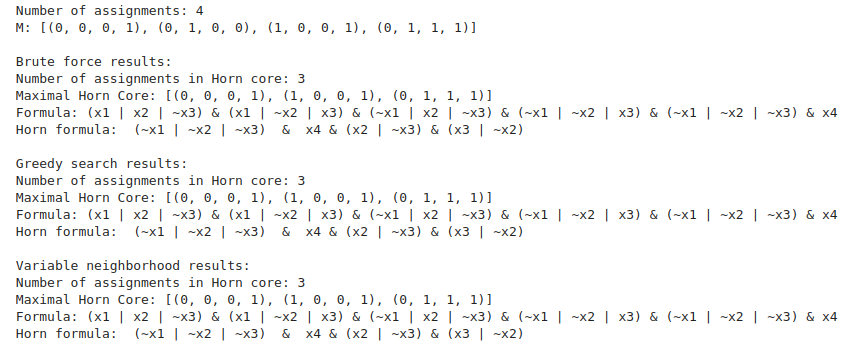
\includegraphics[width=1\linewidth]{small_test_1.png}
    \caption{Rezultati za mali testni skup 1}
    \label{fig:slika1}
\end{figure}

\begin{figure}[H]
    \centering
    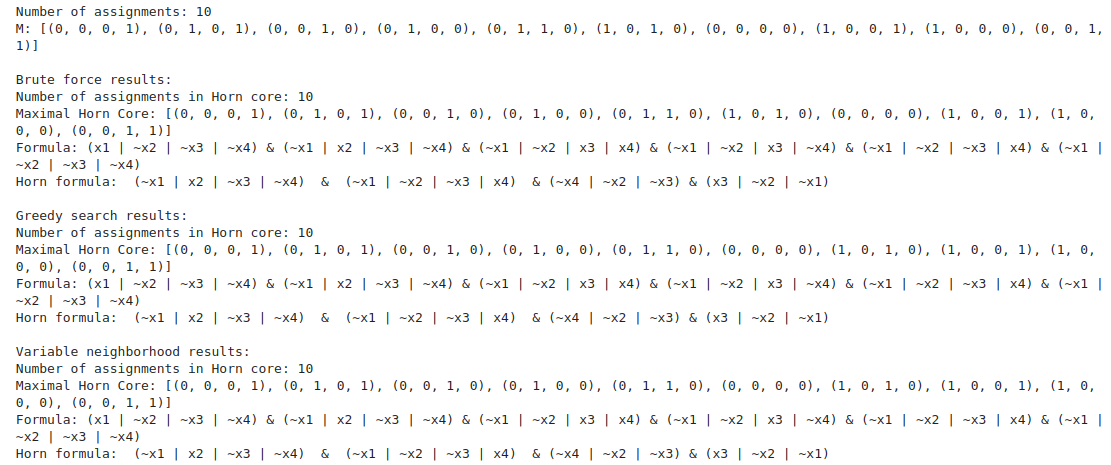
\includegraphics[width=1\linewidth]{small_test_2.png}
    \caption{Rezultati za mali testni skup 2}
    \label{fig:slika2}
\end{figure}

Rezultati testiranja malih testnih skupova su u skladu sa očekivanjima. Rezultati pokazuju da su algoritmi uspeli da pronađu maksimalna Hornova jezgra kako je predviđeno, potvrđujući tačnost i pouzdanost njihovih implementacija. Ovi testovi pružaju osnovu za analizu performansi na složenijim i većim testnim skupovima.

Prethodne studije i teorijska očekivanja sugerišu da bi VNS algoritam trebao da nadmaši pohlepnu pretragu u pronalaženju najvećih Hornovih jezgara. Očekuje se da VNS, zbog svoje sposobnosti da koristi lokalne pretrage i promenljivu strukturu susedstva, pronađe optimalnija rešenja u poređenju sa pohlepnom pretragom. Pohlepna pretraga, iako brza i jednostavna, može praviti kompromise u kvalitetu rešenja zbog svoje determinističke prirode i sklonosti da se zaglavi u lokalnim optimumima. Teorijski, pohlepna pretraga je pogodna za situacije kada je brzina kritični faktor, ali njena sposobnost da pronađe globalno optimalna rešenja je ograničena.

U nastavku su prikazani rezultati testiranja algoritma VNSa i pohlepne pretrage na tri velika testna skupa. Na slikama \ref{fig:test1_greedy_performance}, \ref{fig:test1_vns_performance}, \ref{fig:test2_greedy_performance}, \ref{fig:test2_vns_performance}, \ref{fig:test3_greedy_performance}, i \ref{fig:test3_vns_performance} mogu se videti grafike vremena izvršavanja i veličine Hornovog jezgra ovih algoritama na sva tri testna skupa. Svaka slika omogućava uvid u promene u ukupnom vremenu izvršavanja i veličini najbolje pronađenog jezgra tokom iteracija, što pomaže u analizi efikasnosti i performansi oba algoritma na različitim testnim skupovima. Tabela \ref{tab:test_results} sadrži detaljne rezultate performansi. Ova tabela prikazuje broj modela u testnom skupu, prosečno vreme po iteraciji ($T\_avg$) i ukupno vreme izvršavanja svih 20 iteracija algoritma ($T\_tot)$, kao i prosečnu veličinu najboljeg Hornovog jezgra za sve iteracije algoritma ($Veličina\_jezgra\_avg$) i veličinu najboljeg jezgra pronađenog tokom svih iteracija ($Veličina\_jezgra\_tot$). Veličina jezgra predstavlja broj modela uključenih u to jezgru.


\begin{figure}[H]
    \centering
    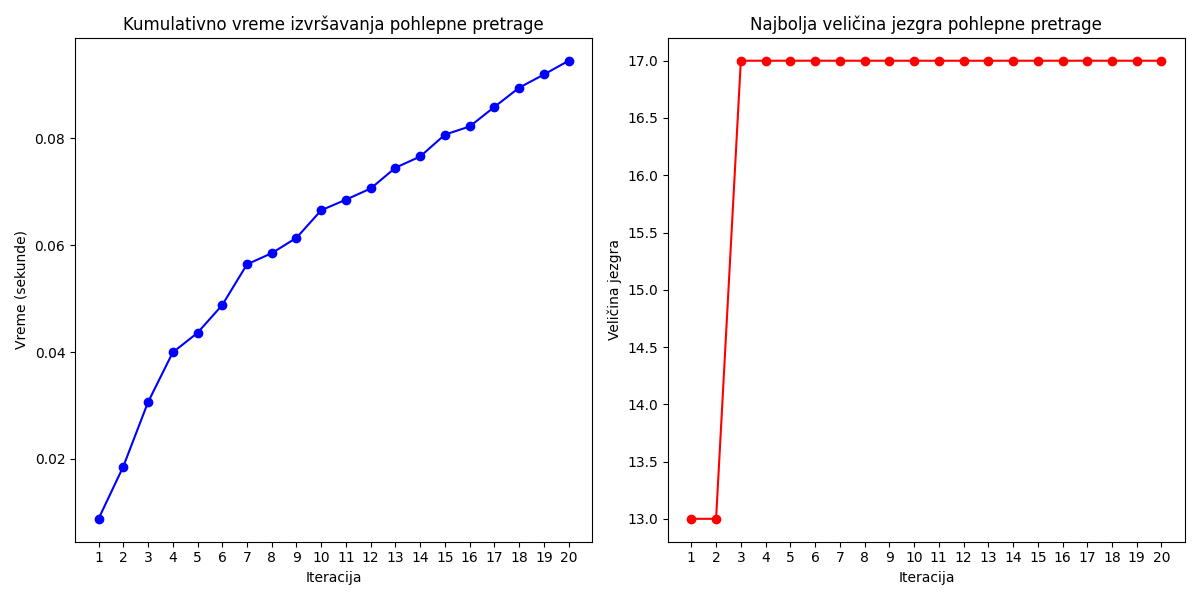
\includegraphics[width=0.8\textwidth]{test1_greedy_performance.png}
    \caption{Grafik vremena izvršavanja i veličine Hornovog jezgra za pohlepnu pretragu na prvom velikom testnom skupu.}
    \label{fig:test1_greedy_performance}
\end{figure}

\begin{figure}[H]
    \centering
    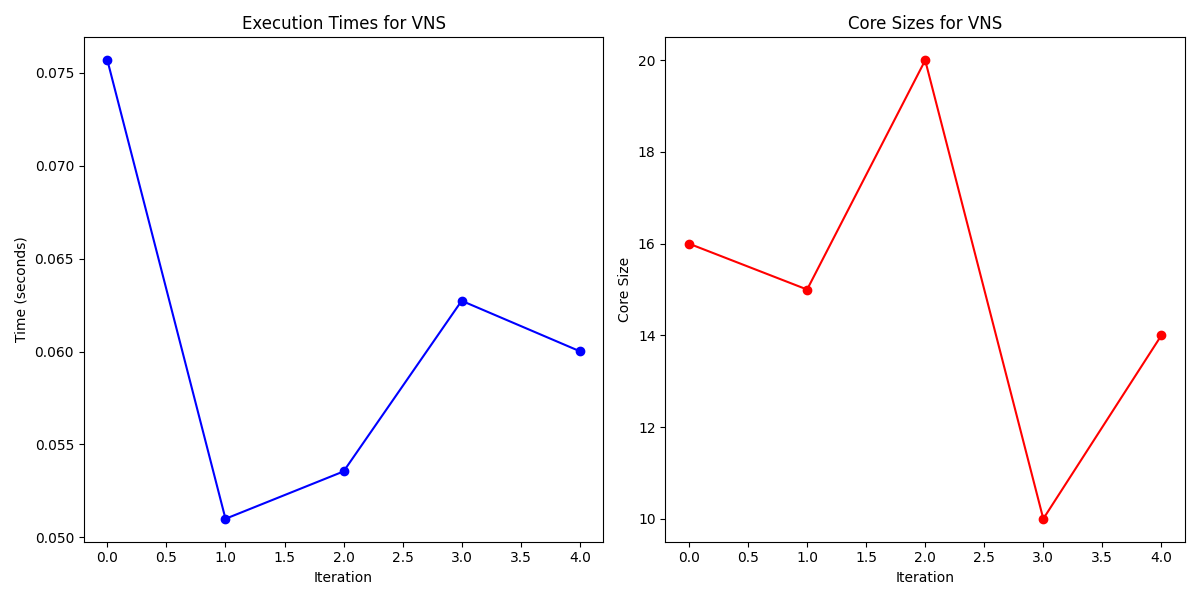
\includegraphics[width=0.8\textwidth]{test1_vns_performance.png}
    \caption{Grafik vremena izvršavanja i veličine Hornovog jezgra za VNS algoritam na prvom velikom testnom skupu.}
    \label{fig:test1_vns_performance}
\end{figure}

\begin{figure}[H]
    \centering
    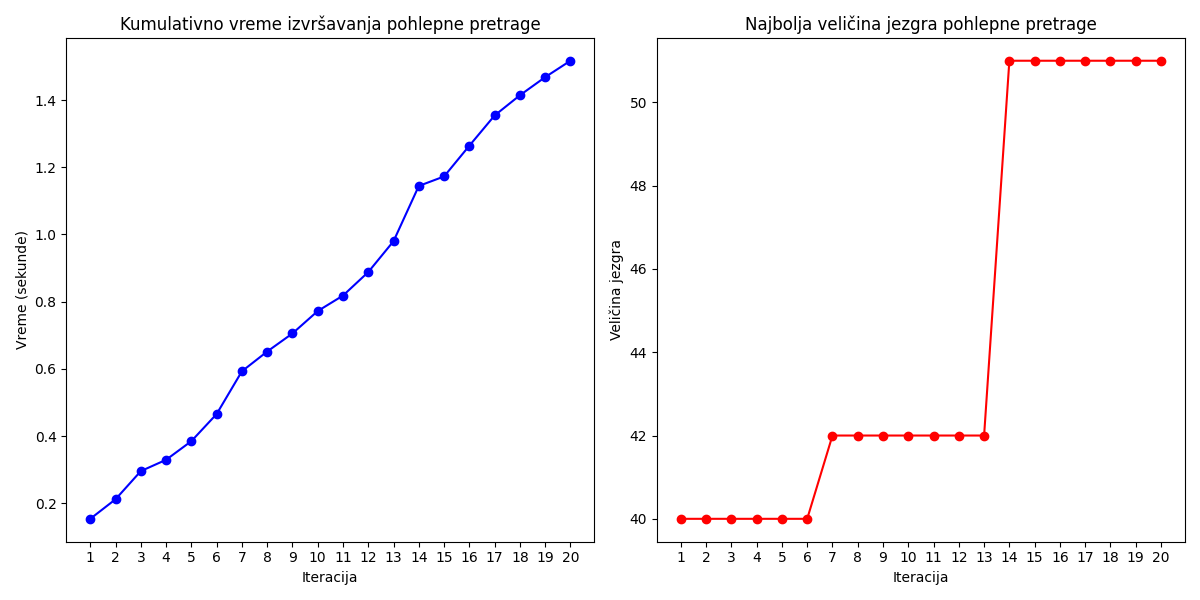
\includegraphics[width=0.8\textwidth]{test2_greedy_performance.png}
    \caption{Grafik vremena izvršavanja i veličine Hornovog jezgra za pohlepnu pretragu na drugom velikom testnom skupu.}
    \label{fig:test2_greedy_performance}
\end{figure}

\begin{figure}[H]
    \centering
    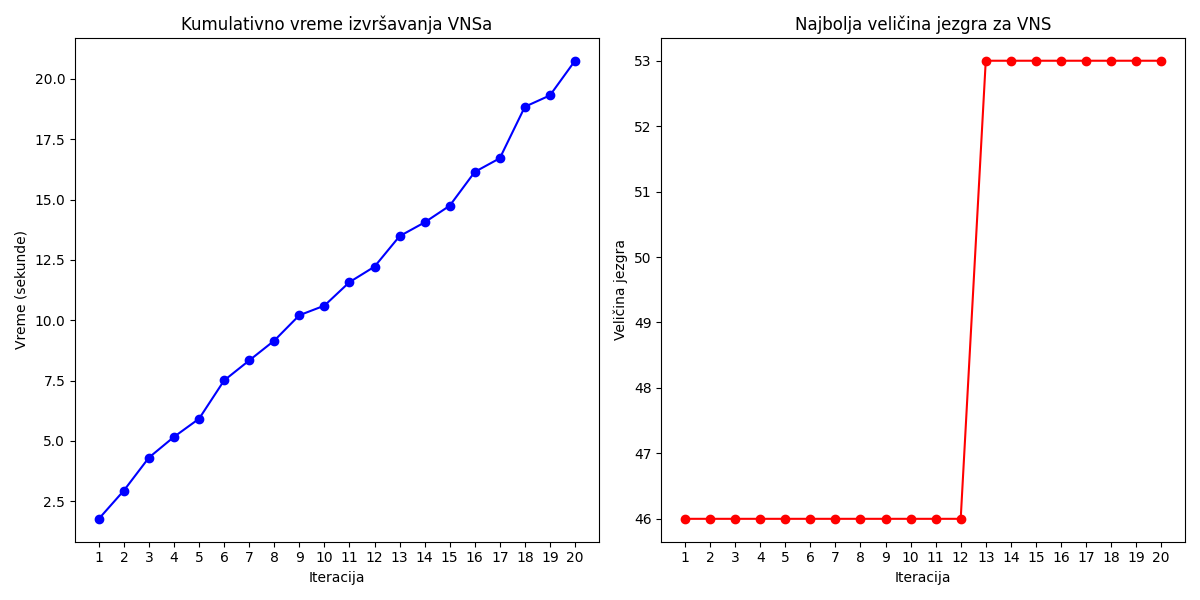
\includegraphics[width=0.8\textwidth]{test2_vns_performance.png}
    \caption{Grafik vremena izvršavanja i veličine Hornovog jezgra za VNS algoritam na drugom velikom testnom skupu.}
    \label{fig:test2_vns_performance}
\end{figure}

\begin{figure}[H]
    \centering
    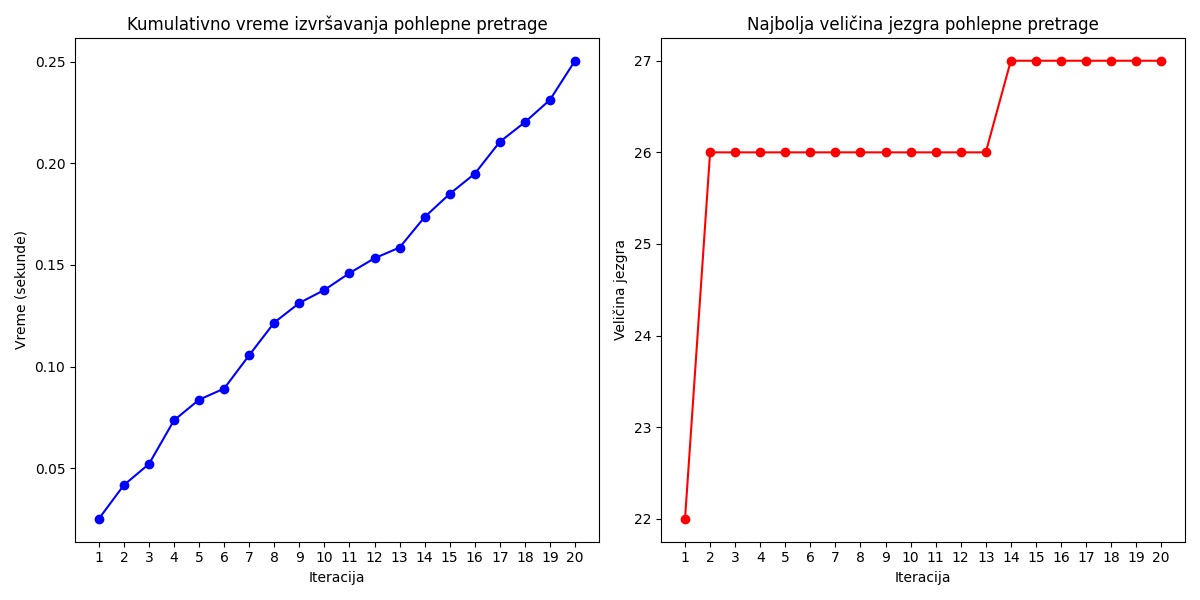
\includegraphics[width=0.8\textwidth]{test3_greedy_performance.png}
    \caption{Grafik vremena izvršavanja i veličine Hornovog jezgra za pohlepnu pretragu na trećem velikom testnom skupu.}
    \label{fig:test3_greedy_performance}
\end{figure}

\begin{figure}[H]
    \centering
    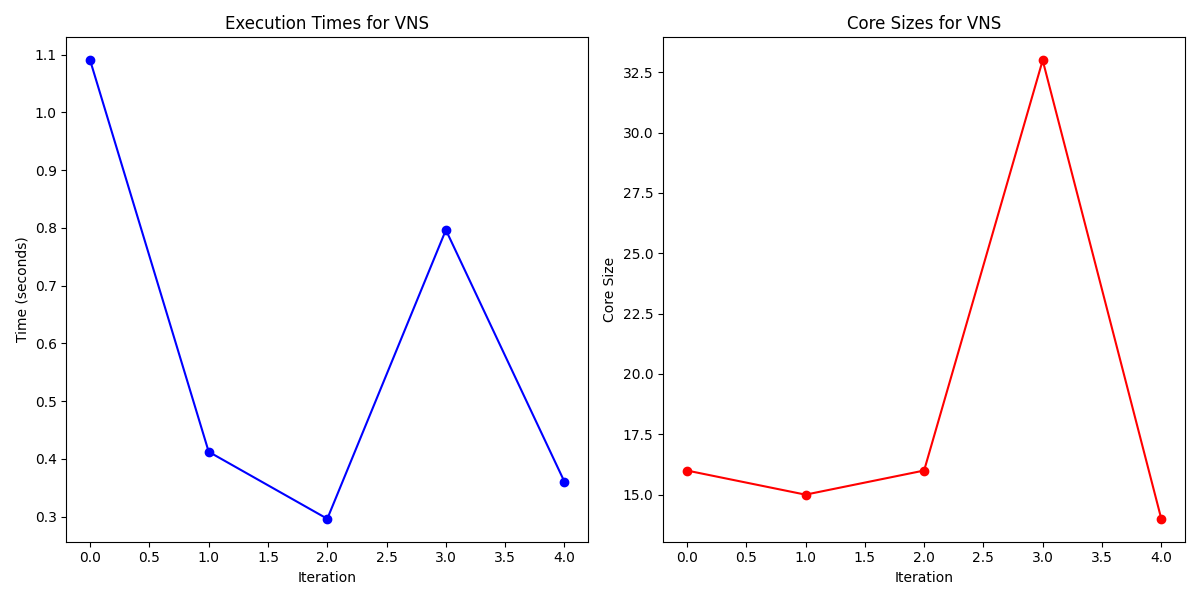
\includegraphics[width=0.8\textwidth]{test3_vns_performance.png}
    \caption{Grafik vremena izvršavanja i veličine Hornovog jezgra za VNS algoritam na trećem velikom testnom skupu.}
    \label{fig:test3_vns_performance}
\end{figure}


\renewcommand{\arraystretch}{2} % Povecava visinu redova
\begin{table}[H]
\centering
\resizebox{\textwidth}{!}{%
\begin{tabular}{|c|c|cccc|cccc|}
\hline
\multirow{2}{*}{\textbf{Test skup}} & \multirow{2}{*}{\textbf{Broj modela testnog skupa}} & \multicolumn{4}{c|}{\textbf{Pohlepna pretraga}} & \multicolumn{4}{c|}{\textbf{VNS}} \\ \cline{3-10} 
 &  & \multicolumn{1}{c|}{\textbf{T\_avg}} & \multicolumn{1}{c|}{\textbf{T\_tot}} & \multicolumn{1}{c|}{\textbf{Veličina\_jezgra\_avg}} & \textbf{Veličina\_jezgra\_tot} & \multicolumn{1}{c|}{\textbf{T\_avg}} & \multicolumn{1}{c|}{\textbf{T\_tot}} & \multicolumn{1}{c|}{\textbf{Veličina\_jezgra\_avg}} & \textbf{Veličina\_jezgra\_tot} \\ \hline
Skup 1 & 93 & \multicolumn{1}{c|}{0.005} & \multicolumn{1}{c|}{0.095} & \multicolumn{1}{c|}{11.3} & 17 & \multicolumn{1}{c|}{0.087} & \multicolumn{1}{c|}{1.742} & \multicolumn{1}{c|}{11.2} & 20 \\ \hline
Skup 2 & 330 & \multicolumn{1}{c|}{0.076} & \multicolumn{1}{c|}{1.517} & \multicolumn{1}{c|}{29.25} & 51 & \multicolumn{1}{c|}{1.038} & \multicolumn{1}{c|}{20.752} & \multicolumn{1}{c|}{31.95} & 53 \\ \hline
Skup 3 & 221 & \multicolumn{1}{c|}{0.013} & \multicolumn{1}{c|}{0.251} & \multicolumn{1}{c|}{20.9} & 27 & \multicolumn{1}{c|}{0.635} & \multicolumn{1}{c|}{12.699} & \multicolumn{1}{c|}{22.25} & 36 \\ \hline
\end{tabular}%
}
\caption{Rezultati na tri velika testna skupa}
\label{tab:test_results}
\end{table}



Rezultati testiranja velikih testnih skupova potvrđuju prethodna očekivanja. VNS algoritam zaista nadmašuje pohlepnu pretragu u pronalaženju većih Hornovih jezgara. Na primer, u testnom skupu 3, VNS je pronašao jezgro veličine 36, dok je pohlepna pretraga pronašla jezgro veličine 27. Ovi rezultati potvrđuju da VNS koristi svoje napredne tehnike pretrage kako bi pronašao globalno bolja rešenja.

Takođe, pohlepna pretraga pokazuje brže vreme izvršavanja, ali često sa većim oscilacijama u kvalitetu rešenja tokom različitih iteracija. Ove oscilacije ukazuju na njenu sklonost da se zaglavi u lokalnim optimumima, što je u skladu sa teorijskim očekivanjima. VNS se, s druge strane, pokazuje kao robustan pristup u pronalaženju rešenja koja pohlepna pretraga može prevideti, što potvrđuje njegovu prednost u preciznosti i stabilnosti rešenja.

Dobijeni rezultatit su u skladu sa postojećim istraživanjima, koji sugerišu da VNS pruža bolje rezultate u pronalaženju globalno optimalnih rešenja. Dok pohlepna pretraga nudi prednosti u brzini i jednostavnosti, prethodne studije su istakle da VNS koristi složenije tehnike za izbegavanje lokalnih optimuma, što je evidentno u njegovoj sposobnosti da dosledno identifikuje veća jezgra u poređenju sa pohlepnom pretragom.

U zaključku, dok VNS pokazuje superiornost u preciznosti, pohlepna pretraga ostaje važan alat zbog svoje jednostavnosti i brzine. Izbor između ova dva algoritma zavisi od specifičnih potreba aplikacije i raspoloživih resursa. Ova analiza omogućava donošenje informisanih odluka o tome koji algoritam koristiti u zavisnosti od specifičnih zahteva problema.

\chapter{Zaključak i pravac daljeg rada}

U ovom radu razmotrena je problematika pronalaženja maksimalnog Hornovog jezgra, koristeći različite algoritme i tehnike za evaluaciju efikasnosti pristupa. Eksperimenti su sprovedeni na malim i velikim skupovima podataka. Analizom su obuhvaćeni kako metaheuristički pristupi, kao što su metoda promenljivih okolina (VNS) i pohlepna pretraga, tako i klasična metoda grube sile. 

Eksperimentalni rezultati su pokazali da metaheuristički algoritmi pružaju značajnu prednost u smislu efikasnosti prilikom obrade velikih skupova podataka, dok pristup grube sile ostaje koristan za male instance zbog svoje tačnosti.
Analizom rezultata na velikim skupovima podataka može se zaključitit da VNS pruža nešto bolje rezultate u poređenju sa pohlepnom pretragom, što ukazuje na njegovu superiornost u ovom kontekstu.

Zaključujeno je da su metaheuristički algoritmi, kao što su metoda promenljivih okolina i pohlepna pretraga, veoma korisni za rešavanje problema maksimalnog Hornovog jezgra zbog svoje sposobnosti da nalaze približna rešenja u razumnom vremenskom okviru.

Razvijeni algoritam za generisanje Horn formula pokazao je zadovoljavajuće rezultate u testiranju, ali postoje mogućnosti za dalja unapređenja. Trenutna verzija algoritma koristi osnovne tehnike za generisanje formula, ali u budućem radu bi moglo biti korisno implementirati sofisticiranije metode koje bi mogle poboljšati kvalitet generisanih formula i ubrzati proces generacije.

Za budući rad, preporučuje se dalja optimizacija postojećih metaheurističkih algoritama kako bi se poboljšala njihova tačnost i brzina, posebno u kontekstu vrlo velikih skupova podataka. Takođe, istraživanje novih metaheurističkih pristupa i njihova komparacija sa tradicionalnim metodama može pružiti dodatne uvide u efikasnost različitih tehnika. Implementacija naprednih tehnika kao što su hibridni algoritmi, koji kombinuju prednosti različitih metaheuristika, mogla bi biti korisna za dalje unapređenje rešenja problema maksimalnog Hornovog jezgra.

Pored toga, uvođenje novih evaluacijskih kriterijuma i testiranje na različitim vrstama instanci može doprineti razumevanju ograničenja i prednosti trenutnih metoda. Takođe, istraživanje mogućnosti primene razvijenih algoritama u drugim sličnim problemima i oblastima može otvoriti nove pravce istraživanja i primene.

Zaključno, ovaj rad pruža značajan doprinos razumevanju i primeni metaheurističkih tehnika za rešavanje kompleksnih problema, kao što je problem pronalaženja maksimalnog Hornovog jezgra. Istraživanje je omogućilo uvid u efikasnost različitih metoda i njihove prednosti i ograničenja. Takođe, pružena su osnova i smernice za buduća istraživanja i unapređenja, otvarajući prostor za dalje inovacije i optimizacije u ovoj oblasti.

% \lstinputlisting[caption=Sample Code Listing C++, label={lst:listing-cpp}, language=C++]{./code1.cpp}
% ------------------------------------------------------------------------------
% \pangrami

% \pangrami

% ------------------------------------------------------------------------------
% Literatura
% ------------------------------------------------------------------------------
\literatura

% ==============================================================================
% Završni deo teze i prilozi
\backmatter
% ==============================================================================

% ------------------------------------------------------------------------------
% Biografija kandidata
\begin{biografija}
  \textbf{Nikola Belaković} je rođen u Kraljevu 14. septembra 2000. godine.
  Išao je u osnovnu školu „Milun Ivanović” u Kraljevu, završio je odličnim uspehom
  i bio nagrađen Vukovom diplomom. Nakon završene osnovne škole
  upisao je prirodno-matematički smer „Gimanzije Kraljevo”.
  Po završetku srednje škole, odlučuje da upiše smer Informatika na Matematičkom fakultetu u Beogradu.
  Osnovne studije završava u roku od četiri godine i upisuje master studije na istom smeru.
  

\end{biografija}
% ------------------------------------------------------------------------------

\end{document}